%% Template originaly created by Karol Kozioł (mail@karol-koziol.net) and modified for ShareLaTeX use

\documentclass[a4paper,11pt]{article}
\usepackage[T1]{fontenc}
\usepackage[utf8]{inputenc}
\usepackage{graphicx}
\usepackage{xcolor}
\renewcommand\familydefault{\rmdefault}
\usepackage{tgheros}
\usepackage[hidelinks]{hyperref}

\usepackage{amsmath,amssymb,amsthm,textcomp}
\usepackage{enumerate}
\usepackage{multicol}
\usepackage{tikz}
%%\usepackage[utf8]{vietnam}
\usepackage[unicode]{hyperref}

\usepackage{geometry}
\geometry{total={210mm,297mm},
left=25mm,right=25mm,%
bindingoffset=0mm, top=22mm,bottom=25mm}

\linespread{1.3}

\newcommand{\linia}{\rule{\linewidth}{0.5pt}}

% custom theorems if needed
\newtheoremstyle{mytheor}
    {1ex}{1ex}{\normalfont}{0pt}{\scshape}{.}{1ex}
    {{\thmname{#1 }}{\thmnumber{#2}}{\thmnote{ (#3)}}}

\theoremstyle{mytheor}
\newtheorem{defi}{Definition}

% my own titles
\makeatletter
\renewcommand{\maketitle}{
\begin{center}
\vspace{2ex}
{\huge \textsc{\@title}}
\vspace{1ex}
\\
\linia\\
\@author \hfill \@date
\vspace{4ex}
\end{center}
}
\makeatother
%%%

% custom footers and headers
\usepackage{fancyhdr}
\setlength{\headheight}{20pt}
\pagestyle{fancy}
\fancyhead{} % clear all header fields
\fancyhead[L]{
 \begin{tabular}{rl}
    \begin{picture}(15,10)(0,0)
    \put(0,-8){
\includegraphics[width=8mm, height=8mm]{graphics/hcmut.png}}
    %\put(0,-8){\epsfig{width=10mm,figure=hcmut.eps}}
   \end{picture}&
	%
\includegraphics[width=8mm, height=8mm]{hcmut.png} & %
	\begin{tabular}{l}
		\textbf{\bf \ttfamily Ho Chi Minh City, University of Technology}\\
		\textbf{\bf \ttfamily Department of Computer Science and Engineer}
	\end{tabular} 	
 \end{tabular}
}
\fancyhead[R]{
	\begin{tabular}{l}
		\tiny \bf \\
		\tiny \bf 
	\end{tabular}  }
\fancyfoot{} % clear all footer fields
\fancyfoot[L]{\scriptsize \ttfamily Application Based Internet of Things}
\rfoot{Page \thepage}
\renewcommand{\headrulewidth}{0.2pt}
\renewcommand{\footrulewidth}{0.2pt}
%



% code listing settings
\usepackage{listings}
\lstset{
    language=Python,
    basicstyle=\ttfamily\small,
    aboveskip={1.0\baselineskip},
    belowskip={1.0\baselineskip},
    columns=fixed,
    extendedchars=true,
    breaklines=true,
    tabsize=4,
    prebreak=\raisebox{0ex}[0ex][0ex]{\ensuremath{\hookleftarrow}},
    frame=lines,
    showtabs=false,
    showspaces=false,
    showstringspaces=false,
    keywordstyle=\color[rgb]{0.627,0.126,0.941},
    commentstyle=\color[rgb]{0.133,0.545,0.133},
    stringstyle=\color[rgb]{01,0,0},
    numbers=left,
    numberstyle=\small,
    stepnumber=1,
    numbersep=10pt,
    captionpos=t,
    escapeinside={\%*}{*)}
}

%%%----------%%%----------%%%----------%%%----------%%%

\begin{document}

\begin{titlepage}
\begin{center}
HO CHI MINH CITY, UNIVERSITY OF TECHNOLOGY \\
DEPARTMENT OF COMPUTER SCIENCE AND ENGINEER
\end{center}

\vspace{1cm}

\begin{figure}[h!]
\begin{center}

\includegraphics[width=3cm]{graphics/hcmut.png}
\end{center}
\end{figure}

\vspace{2cm}


\begin{center}
\begin{tabular}{c}
\multicolumn{1}{c}{\textbf{{\Large Application-Based Internet of Things Report}}}



~~\\

\\
\multicolumn{1}{l}{\textbf{{\Large}}}\\
\\
\textbf{{\Large}}\\

\\
\\

\end{tabular}
\end{center}

\vspace{3cm}

\begin{table}[h]
\begin{tabular}{rrl}
\hspace{5.1cm} 
&\textit{Student: } & Nguyen Dinh Minh\\

\end{tabular}
\end{table}
\vspace{3cm}
\begin{center}
{\footnotesize HO CHI MINH CITY, 12/2021}
\end{center}
\end{titlepage}

%\thispagestyle{empty}
\renewcommand{\contentsname}{Content}
\newpage
\vspace{1cm}
\tableofcontents
\newpage

\section{Introduction}
The application-based IoT system used in this project involves 4 main layers of the standard IoT environment. The abstract view of the system is depicted in Figure \ref{fig:iot-system}, in which the 4 main modules are highlighted in 4 different colors and the communication protocols between them are also included as interconnecting arrows. Communication involves both wireless protocols (depicted as dash arrows) and wired connections (depicted as normal arrows). The names of the communication protocol being used are typed right beside the corresponding arrows. We only have 2 communication protocol in this project: MQTT protocol and UART communication. The implementation of these protocols will further be explain in more detail later.
\begin{figure}
    \centering
    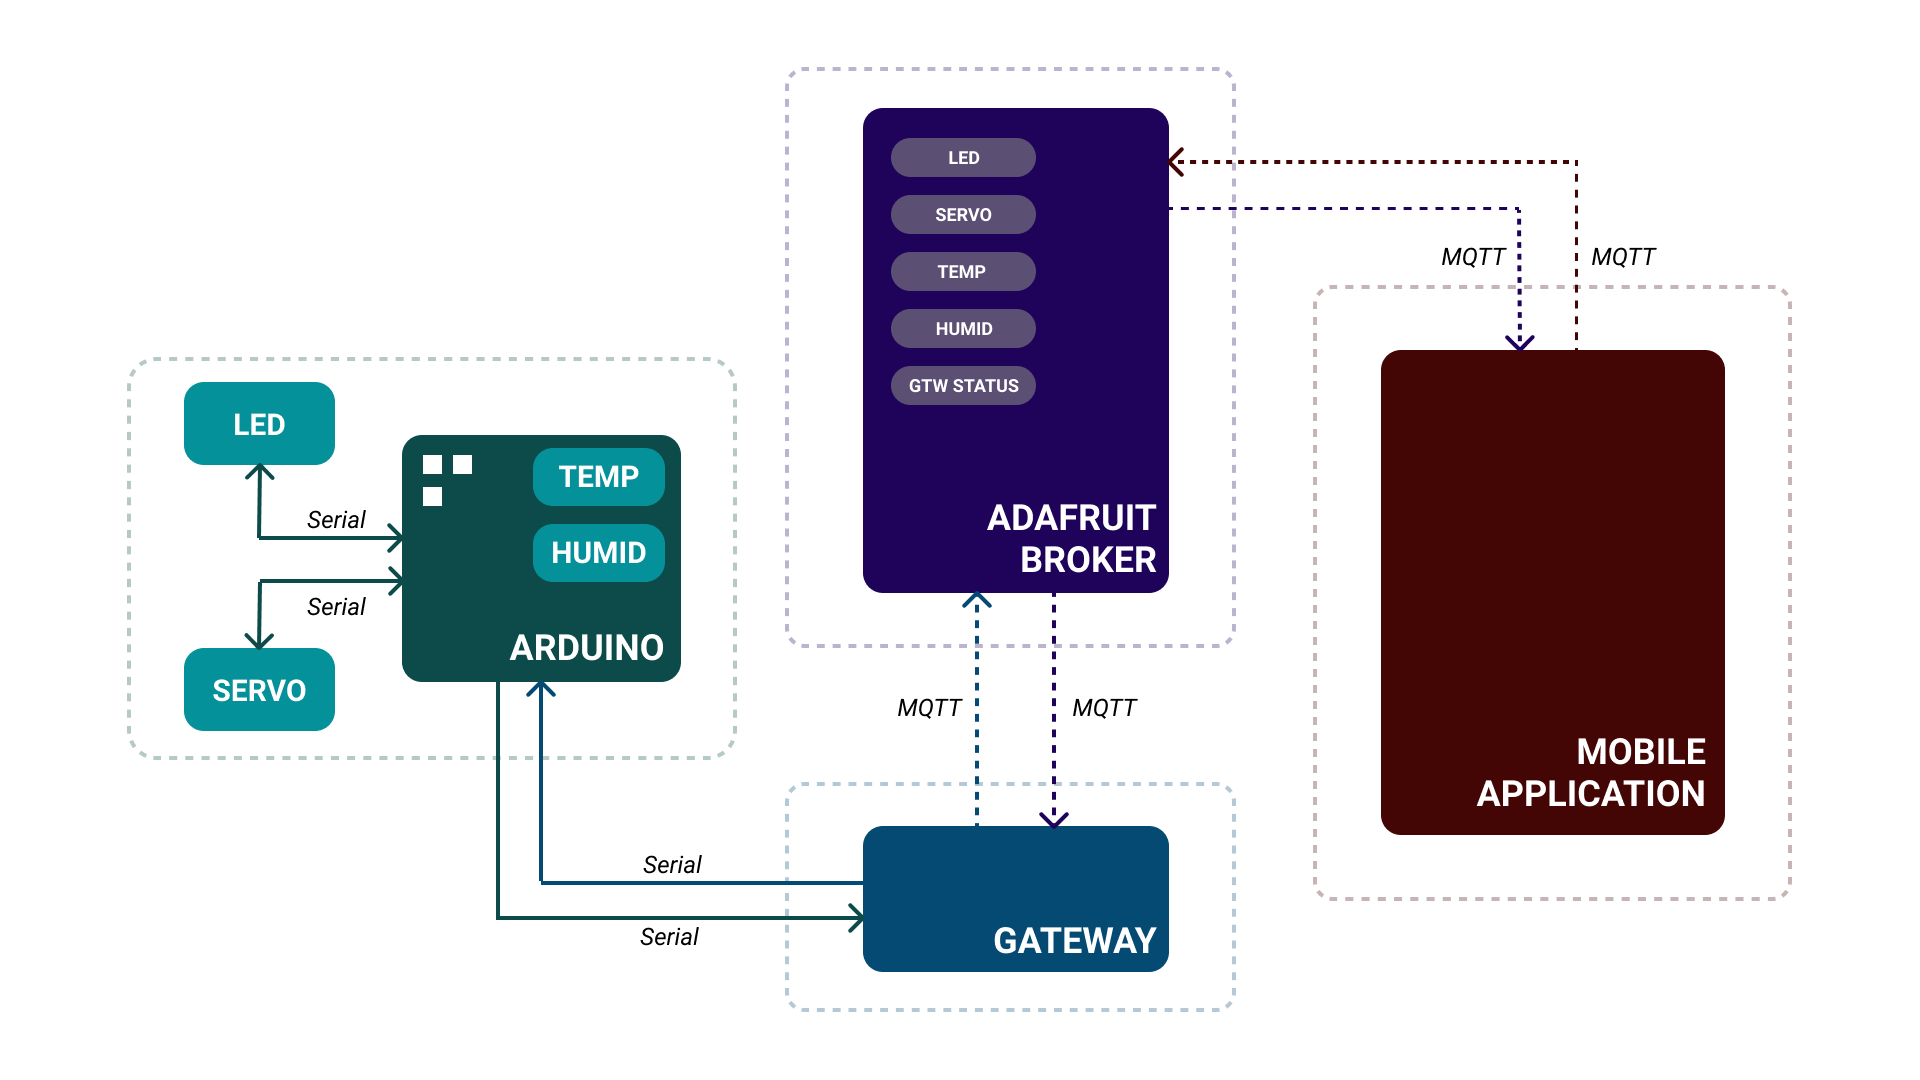
\includegraphics[scale=0.25]{graphics/Overall Architecture.png}
    \caption{IoT System Layers}
    \label{fig:iot-system}
\end{figure}

The first module of our system is the \textbf{Arduino Node}. This layer of the IoT system do the simple assembly work that receives data from the external \textit{Led} and \textit{Servo} device, as well as generates random \textit{Temperature} and \textit{Humidity} value. The \textit{Arduino} is also responsible for sending these data packets through UART communication to the next module, the Gateway layer.

Acting as an intermediate module, the \textbf{Gateway} constantly monitors the incoming data packets from both the Arduino and the Adafruit Broker. Its main job is to handle these data and dispatch (send) them to the correct destination. An additional and important feature of the Gateway is to fetch the latest data from the broker and send them to the Arduino node when it first connect (or reconnect) to the server. The implementation of the Gateway will also be explained in more detail in later part of the document.

The broker used in this project is the service provided by the \textbf{Adafruit IO} cloud. The broker provides enough \href{https://io.adafruit.com/api/docs/mqtt.html#adafruit-io-mqtt-api}{\textcolor{blue}{API implementation}} for MQTTv3.1 standard. Our IoT system will have 5 separate feeds on the server to record and distribute data to any client connecting to the broker. We have the \textit{Gateway} is the first MQTT client by which we publish data packets from the \textit{Arduino Node} to the online feeds. Gateway client also subscribes to several (but not all) necessary topics from the broker to receive request messages from the server. The broker maintains an additional feed called \texttt{gtw-status} that record the current status (\textit{online}/\textit{offline}) of the Gateway. Whenever our Gateway successfully connects to the broker, it will automatically set its status to \textit{online} by publish a short message to this feed. In the event the Gateway is \textbf{willing} to disconnect from the server, it will publish an \textit{offline} message to the status topic before leaving. This will be further explained when we come to the implementation of the Gateway.

The second MQTT client, also the last layer of out IoT system, is the \textbf{mobile application}  module. It is at this layer the users have a decent interface to monitor and interact with the IoT components. Much like the Gateway, our mobile application implements the v3.1 version of the MQTT protocol to communicate with the Adafruit server. The detail of the mobile layer is saved until we come to the section \ref{mobile-application}.

Now that's the overview to the IoT architecture. We now continue to explore how to actually put these modules down in the upcoming sections. Before going on, in order to ease up tracking the implementation, the whole project can be found at this Github \href{https://github.com/hescul/adafruit-simple-iot}{\textcolor{blue}{repository}} hosted by the author of this document.
\clearpage
\section{Arduino Implementation}
All the sensor nodes are boiled down to the Arduino. We have 2 actual sensor simulators: the \textbf{built-in Arduino's led} and the \textbf{servo}. The \textbf{temperature} and \textbf{humidity} data are randomly generated by the Arduino's hardware. Listing \ref{code:arduino-program-part1} provides the first part of the source code for this Arduino program, in which we declare some useful symbolic constants and global variables.

\begin{lstlisting}[language=C++, caption= Arduino Program (part 1), escapeinside={(*}{*)}, label=code:arduino-program-part1]
#include <Servo.h>

const int BUFFER_SIZE = 100; (*\label{code:arduino-program-part1:buff-size}*)
char buff[BUFFER_SIZE];      (*\label{code:arduino-program-part1:buff-array}*)

Servo servo;                 (*\label{code:arduino-program-part1:servo}*)
const int servoPIN = 12;
const int servoMin = 100;
const int servoMax = 180;    (*\label{code:arduino-program-part1:servo-max}*)

const int publishDelay = 20000;   // publish every 20s
unsigned long myTime  = millis();
\end{lstlisting}
We're gonna need a buffer to store the incoming messages sent by the Gateway, so we reserve an array of characters whose length defined by the constant \texttt{BUFFER\_SIZE} (line \ref{code:arduino-program-part1:buff-size} and line \ref{code:arduino-program-part1:buff-array}). Line \ref{code:arduino-program-part1:servo} through \ref{code:arduino-program-part1:servo-max} of the listing are the global variables involved in the control of our \texttt{servo}. We will publish random temperature and humidity value every \texttt{publishDealy} milliseconds, and use the variable \texttt{myTime} to control the delay without actually freezing the big while loop (since the big while loop is also responsible for monitoring the incoming messages).
\begin{lstlisting}[language=C++, caption= Arduino Program (part 2), escapeinside={(*}{*)}, label=code:arduino-part2]
void setup() {
  // setup built in led
  pinMode(LED_BUILTIN, OUTPUT);

  // setup servo
  servo.attach(servoPIN);
  servo.write(servoMin); (*\label{code:arduino-part2:servoMin}*)
  
  // set baud rate
  Serial.begin(9600);

  // seed the PRNG
  randomSeed(analogRead(0));
}
\end{lstlisting}
Now we are ready to define the \texttt{setup()} function, as shown in Listing \ref{code:arduino-part2}. The \texttt{setup()} function is straightforward. We use the symbolic constants defined earlier to setup the built-in LED and the pin that will control the servo. We also make the servo to rotate to the \texttt{servoMin} angle on launch (line \ref{code:arduino-part2:servoMin}). Our servo will only rotate between \texttt{servoMin} and \texttt{servoMax} degree. We then set the baud rate for the serial communication to the default value of Arduino's, which is 9600. The last step is to seed the built-in PRNG from which we will use to generate random integer value in later part of the implementation.

Listing \ref{code:arduino-part3} shows an (over) simplified implementation version of the \texttt{loop()} function.
\begin{lstlisting}[language=C++, caption= Arduino Program (part 3), escapeinside={(*}{*)}, label=code:arduino-part3]
void loop() {
     if (Serial.available() > 0) {
        // read from serial and process the received message
     }
     if (millis() - myTime > publishDelay) {
        // send random temperature and humidity value to Serial
     }
}
\end{lstlisting}
There are 2 events happens inside the forever loop. The first event occurs whenever the \texttt{Serial} instance detects incoming serial data coming from the Gateway. If this is the case, we will start process the character sequence to decode the message. The routine to accomplish this is explained in sub-section \ref{decoding-message}. The second event of the big loop occurs every a fixed amount of time, determined by the \texttt{publishDelay} variable. Currently, as shown in the listing, we are sending data packets to the Serial every 20 seconds. The \texttt{millis()} function is a built-in function that returns the number of milliseconds passed since the Arduino board began running the current program. To establish the 20s-delay inside the loop without hindering the serial's routine, we will utilise this handy function. We constantly ask for the elapsed time, and whenever the period surpassed the value stored in the \texttt{publishDelay} variable, we do the transmitting-data routine, which will be explained in subsection \ref{transmitting-data}.
\clearpage

\subsection{Decoding-Message Routine}
\label{decoding-message}
Listing \ref{code:arduino-part4} shows what happens if a character sequence is detected at the serial.
\begin{lstlisting}[language=C++, caption= Arduino Program (part 4), escapeinside={(*}{*)}, label=code:arduino-part4]
if (Serial.available() > 0) {
    // expected data pactket of the form: !<TOPIC_ENUM>:<VALUE>#
    Serial.readBytesUntil('#', buff, BUFFER_SIZE);
    String payload = String(buff);
    if (payload.length() > 0) {
      int code = payload.substring(payload.indexOf('!') + 1, payload.indexOf(':')).toInt();
      int value = payload.substring(payload.indexOf(':') + 1, payload.indexOf('#')).toInt();
      switch(code) {
      case 0:
        digitalWrite(LED_BUILTIN, (value == 1) ? HIGH : LOW);
        break;
      case 1:
        servo.write(constrain(value, servoMin, servoMax));
        break;
      default:
        break;
      } // !switch
    } // !payload > 0
} // !serial.available()
\end{lstlisting}
We use a method called \texttt{readBytesUntil()} to save the incoming character sequence in the \texttt{buff} array. We terminate the reading whenever we hit a \#, as it marked the end of the message sequence. Having read the message as a C-style string, we construct a String instance for it and save the newly constructed object to the \texttt{payload} variable. The use of String here is to simplify further manipulation on the message sequence since the Arduino offer rich methods to handle String than that of raw C-style string.

It may seem redundant, but the first \texttt{if} coming right after the first string processing is to ensure we are not digging in an empty string, since we are about to invoke some expensive methods. We start off extracting the enumerated code that encodes the node that this message is targeting. It should be (for this moment) either the LED or the servo node. We will use 0 for LED and 1 otherwise. The next step is to extract the the data value that the Gateway wishes to enact on the target node and save it to the \texttt{value} variable. When done, we can happily use a simple \texttt{switch} statement on the \texttt{code} variable and process on according matches.\\ \\
\clearpage

\subsection{Transmitting-Data Routine}
\label{transmitting-data}
The following listing shows the activities happening every 20s-delay.
\begin{lstlisting}[language=C++, caption= Arduino Program (part 5), escapeinside={(*}{*)}, label=code:arduino-part5]
if (millis() - myTime > publishDelay) {
    myTime = millis();  // reset current time
    // using data frame of the form: !<ID>:<topic_name>:<data>:#
    Serial.print("!1:temperature:" + String(random(0, 100)) + "#");
    Serial.print("!1:humidity:" + String(random(0, 100)) + "#");
}
\end{lstlisting}
The code is straightforward. Whenever we hit the 20s interval, we reset the \texttt{myTime} variable to the current amount of elapsed time, and then start sending 2 random value (invoked through the \texttt{random()} function) for temperature and humidity.

Now that we've done with the first layer of our IoT system. The full implementation of this module can be found under the folder named \textit{arduino-node} inside this Github \href{https://github.com/hescul/adafruit-simple-iot}{\textcolor{blue}{repository}}.
\clearpage
\section{Gateway Implementation}
Things start to get more interesting and complicated here. The Gateway will have to implement both the MQTT protocol and UART communication, using Python. For the MQTT, in order to keep the project consistent, we will use the \href{https://pypi.org/project/paho-mqtt/}{\textcolor{blue}{paho-mqtt}} package to establish the communication protocol. For the UART serial, we will stick with the popular \href{https://pypi.org/project/pyserial/}{\textcolor{blue}{pyserial}} package.

\subsection{Gateway Overture}
\label{subsection:gtw-overture}
Before getting our hands dirty into the implementation of the Gateway, there are plentiful of things to discuss. We will devote this part of the Gateway section for sketching out the overall activities of our gateway program, as well as explaining some observations of the MQTT on Adafruit server.

\subsubsection{Gateway Features}
The bulk of this python program is to running a simple gateway that is capable of receiving data from the \href{https://io.adafruit.com/}{\textcolor{blue}{Adafruit server}} (broker) and dispatching it to an IoT Arduino node. The gateway also monitors the data sent from the Arduino and publishes it to the server, therefore establishing a form of communication between the broker and the sensor. The attributes of this simple implementation of our gateway are listed bellow.
\begin{itemize}
    \item The gateway receives \textbf{temperature} and \textbf{humidity} data from the Arduino and publishes them to the broker.
    \item The gateway listens to \textbf{led} and \textbf{servo} data from the broker and dispatches them to the Arduino.
    \item The gateway is in charge of the \textbf{gtw-status} topic, which is exclusively reserved for the gateway to declare its status to the broker.
    \item The gateway also maintains a concrete connection with the Arduino. When launch, the gateway must ensure it has successfully communicated with the Arduino before establish the broker-connection. During runtime, if the arduino connection is compromised, the gateway will immediately terminate it activities, cut off its connection with the broker, do any necessary clean-up work, and exit with a warning.
    \item Whenever the gateway makes a successful connection to the broker, whether it is the first time the gateway connects to the server or it is a re-connection attempt due to any failure, it will automatically fetch the latest data from any topic it subscribes to and dispatch them to the Arduino.
\end{itemize}
With these features kept in mind, we can sketch out the behaviour of our gateway activities. The step-by-step implementation will be further demonstrated in later part of this section. In the mean time, it is not redundant to mention some "catches" when we use the Adafruit server in join with the paho-mqtt package.

\subsubsection{Adafruit Limitation}
MQTT is one of the powerful communication protocols, especially in the world of IoT. Since its invention in 1999, the latest MQTT version one can use at the point of writing this document is \href{https://docs.oasis-open.org/mqtt/mqtt/v5.0/mqtt-v5.0.html}{\textcolor{blue}{MQTT v5.0}}. While we can exploit many rich IoT features provided by the latest version of MQTT, that is not the case for the Adafruit broker, which by far supports just the MQTT v3.1.1. Even this version of MQTT is strong enough to handle almost any asspect of IoT communication, the Adafruit broker isolates itself from the standard and provides its own python \href{https://pypi.org/project/adafruit-io/}{\textcolor{blue}{API library}} for the end users. This API package is built as a wrapper of the paho-mqtt library, made possible by the people behind the Adafruit broker, to provide ease of use and discard the features of the standard that the Adafruit server is not capable of. So basically, if we use the paho-mqtt package to implement the MQTT and not the exclusive library offered by the Adafruit developers, some functionality provided by the library will not take effect. This is one significant point that need be kept in mind when doing paho-mqtt in joint with the Adafruit broker.

So what is missing from the Adafruit server? The comprehensive document (published by the Adafruit, of course) can be found \href{https://io.adafruit.com/api/docs/mqtt.html#adafruit-io-mqtt-api}{\textcolor{blue}{here}}. They provide us with the guide to implement MQTT communication to the Adafruit server without using the exclusive package. There are many points to be considered, for example the limit of the rate of publishing messages, the must of unique client ID, the data packet format,... When doing MQTT with Adafruit server, it is best to follow the instructions in the published document to avoid undefined behaviour, or worse, account banning.

Why not using the exclusive library in the first place? As stated before, we need to keep the project consistent, because later on, we will have to use the paho-mqtt implementation anyway when we reach the last layer of our IoT system. What's more, the use of paho-mqtt is easy for future upgrade and scalability. We may want to switch to another modern broker other than Adafruit, and using the versatile package will not prevent us from doing so. In other words, we only explore a subset of what the paho-mqtt has in store for us, and we should aware of what the Adafruit broker is incapable of, for instance the \textit{retained message} feature.  

\subsubsection{The Clean Session Problem}
What is a clean session? When a client makes a connection to the broker, the client can make a decision whether its information should be remembered by the server. If the client chooses to have its information discarded by the broker (hence the connection session is clean), the server will not store any subscription information or undelivered messages for the client. This way of connection is sometimes called \textit{non-persistent} connection, and is the connection type of choice for those clients that only publish data to the server. For those clients, on the other hand, that subscribe to some topics on the server, the MQTT provides a \textit{persistent} connection, in which the broker will keep the information of the client (the client must provide a \textit{client ID} so that the server can tell apart different clients).

The connection type, whether it is persistent or non-persistent, is up to the developer who implements the MQTT client object. The Adafruit server supports this feature, with a warning up ahead:
\begin{quote}
    Connecting to Adafruit IO via MQTT and reusing the client ID of an existing connection will result in immediate disconnection of the other MQTT client. The MQTT specification requires that "each client connecting to the server has a unique ClientId." \href{http://docs.oasis-open.org/mqtt/mqtt/v3.1.1/csprd02/mqtt-v3.1.1-csprd02.html#_Toc385349767}{\textcolor{blue}{link}}
\end{quote}
So if one opts to make her clients connection "unclean", then she has to look out for indistinguishable client IDs; otherwise, some of the clients will not make it to the Adafruit broker.

The clean session problem is mentioned here because it related to a more powerful feature of the MQTT protocol: the \textit{retained message} feature. The retained message will only work for clients that set their clean session status to false. When a message published to a topic is retained, the broker will mark it as the latest data of that topic and will automatically publish that message to any persistent client reconnecting to the broker who previously subscribed to that same topic. Put it another way, if a client wants to fetch latest data (using the MQTT way) when it makes a successful connection to the server, the client must first need to be a \textbf{persistent client} and subscribe to topics of interest with \textbf{QoS = 1}. Any message that wants to get automatically published by the broker to the client statisfied these 2 requirement will also need be set as \textbf{retained} when published to according topic. The broker will only store the latest retained message for a topic and use it as the latest data. Retain makes writing basic MQTT-only Internet of Things clients easier, without it, a client that connects and subscribes to a feed topic has to wait until a new value is published on the feed to know what state it should be in.

This service provided by the MQTT protocol is just wonderful to use in place of the traditional HTTP routines, but unfortunately, the Adafruit server is not capable of implementing retained message, or, not implementing it the standard way:
\begin{quote}
    Among other factors, our scale, Adafruit IO's mix of MQTT & HTTP APIs, the speed at which we’re taking in new data, and the fact that we’re already storing almost every message that is sent mean that a “simple” feature like retain becomes difficult to support without making MQTT service performance worse for everyone.
\end{quote}
This means if we follow the same way use the retain service discussed above, in the case of Adafruit server, nothing will take effect. However...

\subsubsection{The Retained Message Solution}
The Adafruit does provide a solution for the retained message limitation, as this is one of the essential features of an IoT system. Using this solution, we will NOT gain the functionality of retain though, but we still get the latest message data without touching any HTTP protocol: the use of \textbf{*/get topic}:
\begin{quote}
    For any given Adafruit IO MQTT feed or group, subscribe to the appropriate topic using the feed or group key, then add /get to the topic you subscribed to and publish anything to that new topic (our Arduino library uses the null character). IO will immediately publish, just for that client, the most recent value received on the feed.
\end{quote}
And that's that. If we want any latest piece of data belong to any topic, we just simply subscribe to that topic and publish an empty message to the topic whose name is the said topic appended "/get". The client will immediately receive the latest data from the Adafruit server. However, there is a catch! The use of */get topic is not working for persistent connection. If a persistent client publishes to a /get topic, an undefined behaviour will occur. In other words, when working with Adafruit server, we should ignore the existence of the clean session service and leave it set as default (non-persistent) to avoid weird outcome.

Okay, with these knowledge at hands, we are ready to step into the gateway program implementation. As usual, the full code is sitting under the folder named \textit{gateway} in this Github \href{https://github.com/hescul/adafruit-simple-iot}{\textcolor{blue}{repository}}.

\subsection{Step-by-Step Implementation}
The code is presented as listings, and only those that need explained will be included.
\subsubsection{Setup Part}
It is always a best practice to define and use symbolic constants instead of "magic" data. Listing \ref{code:gtw-initial} shows the initial part of our gateway program.
\begin{lstlisting}[language=Python, caption= Gateway Program - Initial Setup, escapeinside={(*}{*)}, label=code:gtw-initial]
import paho.mqtt.client as mqtt
import time, queue, serial, threading
from serial.serialutil import SerialException
import serial.tools.list_ports as serialtool

# ------- CONFIGURATIONS & CONSTANTS SETUP ------------
# Broker Configurations
HOST_NAME = "io.adafruit.com"   # using Adafruit IO server
HOST_PORT = 8883                # secure connection
USERNAME  = "***"       # replace with actual broker username 
PASSWORD  = "***"       # replace with actual authentication password

# Gateway Configurations
GATEWAY_ID  = "GTW002"
GROUP_KEY   = "iot-lab"     (*\label{code:gtw-initial:group-line}*)
PUB_QOS = 1
SUB_QOS = 1
STAT_TOPIC  = "gateway-status"
SUBSCRIBE_TOPICS = [        (*\label{code:gtw-initial:sublist-line}*)
    "arduino-led",      # record led status
    "arduino-servo",    # record change in servo angle
    STAT_TOPIC          # listen to disconnect signal from the broker
]
SCAN_DELAY  = 1.0
TIME_OUT    = 5.0       # maximum waiting time for blocking
MAX_FAILED_ATTEMPTS = 3     (*\label{code:gtw-initial:max-failed-line}*)

# Devices Configurations
BAUDRATE    = 9600    # Arduino default baudrate
COM_TOKEN   = 'USB Serial Device'


# ---------------------- COLOR CODES --------------------
class col:
    cdtag   = '\033[35;1m'
    mestag  = '\033[1;34m'
    pubtag  = '\033[31;1m'
    subtag  = '\033[0;33m'
    good    = '\033[92m'
    bad     = '\033[31m'
    user    = '\033[0;95m'
    topic   = '\033[1;37m'
    message = '\033[0;94m'
    stage   = '\033[0;93m'
    esc     = '\033[0m'
\end{lstlisting}
The majority of the symbolic constants in the listing are self-explained by their names. Here we have a \texttt{col} class which is used to highlight the debug messages, as shown in Figure \ref{fig:gtw-connection-failed}. Each debug message has a preceding tag key to make it stand out. We are having a problem here. The broker refuses to grant our client access to the server, as told by the red lines. Notice that the lines in red were not hard-coded. Each unsuccessful attempt to the broker has a reason message associated with it, and the paho-mqtt API provides us with a utility method \texttt{connack\_string()} to get the descriptive cause of the failure. The use of this method is saved until we reach the \texttt{callbacks} implementation.

It is worth mentioning that we are making 3 attempts to connect to the server before exiting the program. The constant \texttt{MAX\_FAILED\_ATTEMPTS} at line \ref{code:gtw-initial:max-failed-line} determines this number of retrying attempts. Another interesting point is that the topics involved in our IoT system belong to a \textit{group} of topics called \textbf{iot-lab} (line \ref{code:gtw-initial:group-line}). The use of group will be further explained in section \ref{section:server}. Right now we should focus on the list of subscribe topics at line \ref{code:gtw-initial:sublist-line}. Because we are listening to the LED and servo topics (as described in subsection \ref{subsection:gtw-overture}), we should include their topic name into this list. Notice that the \textbf{gtw-status} topic is included using another symbolic constant. This will come in handy later, since we treat this topic different from the others. This will also be explained until we reach the later part of our gateway implementation.

\begin{figure}
    \centering
    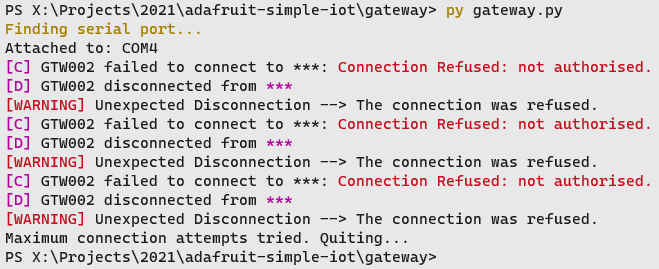
\includegraphics[scale=0.8]{screenshots/connection_failed.png}
    \caption{Connection Failed: Not Authorised}
    \label{fig:gtw-connection-failed}
\end{figure}

Let us run the program again, but this time without the connection of the Arduino as COM port 4. The result is depicted in Figure \ref{fig:gtw-no-com}. Our gateway complains that it found no attached device at the terminal end, so it quits immediately. Later on we will see that, any unexpected disconnection between the gateway and the Arduino will cause our program to terminate without hesitation.

\begin{figure}
    \centering
    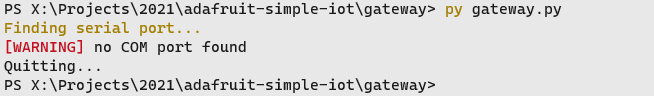
\includegraphics[scale=0.8]{screenshots/no_com.png}
    \caption{No COM port found}
    \label{fig:gtw-no-com}
\end{figure}

\subsubsection{Global Variables and Shared Variables}
\begin{lstlisting}[language=Python, caption= Gateway Program - Variables, escapeinside={(*}{*)}, label=code:gtw-variables]
# ---------- GLOBAL VARIABLES ---------------
block       = False # flag to block thread
exquit      = False # flag to raise disconnect interrupt
greeting    = True  # indicate if this is the first connection
reinit      = False # flag to call init() procedure on reconnect
texceed     = False # indicate if we've reached maximum blocking time
failcount   = 0     # count attempts on fail activity
msg         = ''    # hold buffer message read from serial

# ----------- SHARED-MEMORY -----------------
messageBuffer = queue.Queue()   # holds incoming messages
devicesBuffer = queue.Queue()   # holds outgoing messages
terminate     = False   # control thread termination
scanning      = False   # flag to indicate initial setup
timerexit     = False   # control timer termination
\end{lstlisting}
The next part of our program is reserved for declaring the global and shared variables, as Listing \ref{code:gtw-variables} shows. We have quite a lot variables here, each has it own responsibility on certain aspect of the program, though most of them are involved in the controlling of asynchronous threads. Why thread? The paho-mqtt API offers multiple callbacks that get automatically invoked after a certain action of the MQTT protocol. These threads are, however, asynchronous to the main thread of our program, so we will need these variables to prevent messy debug messages on the console.

Aside from the variables, we have 2 instances of type \texttt{queue} acting as buffers. These queues will ease up the rate of transmitting data and handle multiple incoming messages without hindering other activities in the big while loop. It is important to note that the rate of transmission is NOT unlimited when it comes to Adafruit server:
\begin{quote}
    Adafruit IO's MQTT server imposes a rate limit to prevent excessive load on the service. If a user performs too many publish actions in a short period of time then some of the requests will be rejected and an error message will be published on your /throttle topic. The current rate limit is at most 30 requests per minute for free accounts, 60 per minute with an IO+ account, and expandable via Adafruit IO+ Boost applied to your account.
\end{quote}
You heard the IO, we must have some control in the case the Arduino sends too many data packets in a mimute. The \texttt{deviceBuffer} queue will hold these messages from the Arduino. The Arduino can flood this queue with as many data packets as it wants, because our Gateway program will process these data from the queue one by one independent of the Artduino rate, thus controlling the rate of publishing to the server. On the other hand, the \texttt{messageBuffer} will take on the job of holding messages published by the broker. Its purpose is the same as of the \texttt{deviceBuffer}: prevent the contention occurs inside the big while loop.

\subsubsection{Defining Callbacks}
We will need to define some callbacks that are part of the MQTT API protocol. Some of them serve as debugging, while the others are essential to the gateway functionality. Listing \ref{code:gtw-on-connect} shows the definition of the \texttt{on\_connect()} callback.
\begin{lstlisting}[language=Python, caption= Gateway Program - on\_connect(), escapeinside={(*}{*)}, label=code:gtw-on-connect]
def on_connect(client, userdata, flags, rc):
    if rc != 0: # connection failed
        print(f"{col.cdtag}[C]{col.esc} {GATEWAY_ID} failed to connect to {USERNAME}: {col.bad}{mqtt.connack_string(rc)}{col.esc}")
    else:       # connect successfully
        global greeting
        if greeting:    # the first time this client get connected
            print(f"{col.cdtag}[C]{col.esc} {GATEWAY_ID} connected to {col.user}{USERNAME}{col.esc} with result: {col.good}{mqtt.connack_string(rc)}{col.esc}")
            greeting = False
            global block
            block = False
        else:           # client is making re-connection attempt
            print(f"{col.cdtag}[C]{col.esc} Reconnected to {col.user}{USERNAME}{col.esc} with result: {col.good}{mqtt.connack_string(rc)}{col.esc}")
\end{lstlisting}
The passed in argument \texttt{rc} is used to check the status of connection. If the client failed to connect to the server (\texttt{rc != 0}), then we print out the reason of failure using the method \texttt{connack\_string()} to interpret the reason code. If everything is fine, we continue to see whether the client is making the first connection or a re-connection attempt, and process accordingly.

\begin{lstlisting}[language=Python, caption= Gateway Program - on\_disconnect(), escapeinside={(*}{*)}, label=code:gtw-on-disconnect]
def on_disconnect(client, userdata, rc):
    print(f"{col.cdtag}[D]{col.esc} {GATEWAY_ID} disconnected from {col.user}{USERNAME}{col.esc}")
    if rc != 0:
        print(f"{col.bad}[WARNING]{col.esc} Unexpected Disconnection --> {mqtt.error_string(rc)}")
        global failcount, reinit, scanning
        reinit = True       # the program should do the reinit when get reconnect
        scanning = False    # terminate all activites in the big while loop
        failcount = failcount + 1   # count retrying attempts
\end{lstlisting}
In contrast, Listing \ref{code:gtw-on-disconnect} shows the routine that get called when our client disconnects from the broker. If the disconnection were unexpected (network drops, etc), then we would expect the program to reconnect to the server after a while. The \texttt{reinit} and \texttt{scanning} flag are set to reflect this expectation. We also count the consecutive fail attempts inside this callback for making termination decision on other part of the program.

The next callback shall be the \texttt{on\_message()}, represented in Listing \ref{code:gtw-on-message}. This time we utilize the argument \texttt{userdata} which is automatically passed in by the MQTT implementation. The \texttt{userdata} is an object reserved for whatever purpose the developers want to pass custom data into callbacks that accept the argument. Here, we will use it to filter out the owning messages (messages that are sent and received by the same client). Before publishing any message to the server, we set the \texttt{userdata} object to hold an array of string where the first string is the payload and the second string is the topic name. This instance of the \texttt{userdata} object will then get passed into any callback that has a parameter accepting the object, including our \texttt{on\_message()} callback. It is then the job of the \texttt{on\_message()} function to use the passed in argument to check if the received message is the same as one hold by the \texttt{userdata}.
\begin{lstlisting}[language=Python, caption= Gateway Program - on\_message(), escapeinside={(*}{*)}, label=code:gtw-on-message]
def on_message(client, userdata, message):
    msgv = message.payload.decode()                         # get message value
    msgt = message.topic[message.topic.find('.') + 1:]      # get message topic
    # filter out owning message
    if msgv == userdata[0] and msgt == userdata[1]:
        global block    # release block
        block = False
    else:
        print(f"{col.mestag}[M]{col.esc} Received {col.message}{msgv}{col.esc} on topic: {col.topic}{msgt}{col.esc}")
        # if receive offline instruct from the broker
        if (msgt == STAT_TOPIC and msgv == "offline"):
            global exquit
            exquit = True
        
        # otherwise add message to the buffer
        else:
            if scanning: messageBuffer.join()
            messageBuffer.put((msgt, msgv))
\end{lstlisting}
The listing reveals more than just the filtering-message thing. Here we also handle the case where we receive an \textbf{offline} message from the topic \textbf{gtw-status}. The flag \texttt{exquit} is set to indicate we should clean up and terminate our program.

The 2 last callbacks involving in this program are shown in Listing \ref{code:gtw-on-pubsub}. For the publishing, we just simply check the topic we are sending message to and change the debug message accordingly. The subscribing, on the other hand, has a job to release the thread lock hold by the variable \texttt{block}. Why blocking thread? This has to do with the order that the debug messages appear on the console. Normally, the subscribing protocol is very fast and less error-prone, so the subscription message will usually get printed first, even before the successful connection message get printed. Blocking is put in here to make the debug console more intuitive.
\begin{lstlisting}[language=Python, caption= Gateway Program - on\_publish() and on\_subscribe(), escapeinside={(*}{*)}, label=code:gtw-on-pubsub]
def on_publish(client, userdata, mid):
    if "get" in userdata[1]:
        print(f"Fetching {col.stage}latest data{col.esc} from {userdata[1][:-4]}...")
    elif userdata[1] is STAT_TOPIC:
        print(f"{GATEWAY_ID} has set its status to {col.stage}{userdata[0]}{col.esc}")
    else:
        print(f"{col.pubtag}[P]{col.esc} Published {col.pubtag}{userdata[0]}{col.esc} to: {col.topic}{userdata[1]}{col.esc}")

def on_subscribe(client, userdata, mid, granted_qos):
    global block
    print(f"{col.subtag}[S]{col.esc} Subscribed to: {col.topic}{userdata}{col.esc}")
    block = False   # release block
\end{lstlisting}

Before moving on, let see how a successful connection to the server looks like. Figure \ref{fig:gtw-normal} illustrates a normal gateway connection. We start off finding the COM port where the Arduino attachs to, and then try to establish a connection to the server. On successful connection, we start fetching latest data from the topics in the subscribe list. Finally, we publish an \textbf{online} message to the \textbf{gtw-status} topic before jump into the forever while loop.

\begin{figure}
    \centering
    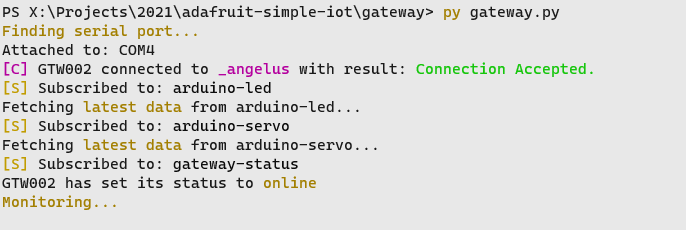
\includegraphics[scale=0.8]{screenshots/normal.png}
    \caption{A successful gateway connection.}
    \label{fig:gtw-normal}
\end{figure}

\subsubsection{Utility Functions}
Let's talk a little bit about some helpful functions used throughout the program. There are quite a lot of them, but the document only lists those that worth mentioning. Listing \ref{code:gtw-init} shows the \texttt{init()} routine, which is responsible for subscribing to the required topics and getting latest data upon each successful subscription. This function will also come in handy when our client get unexpected disconnection and then wish to resubscribe to the topics after reconnecting to the server. The function also illustrates the use of \texttt{userdata} object, the */get solution for latest data fetching, and the variable \texttt{block} to synchronize debug message. The function finishes off setting the gateway status to \textbf{online} by publishing the according message to the \texttt{STAT\_TOPIC}.
\begin{lstlisting}[language=Python, caption= Gateway Program - init() function, escapeinside={(*}{*)}, label=code:gtw-init]
def init():
    global gtw, ser
    # subscribe to required topics
    # -----
    for top in SUBSCRIBE_TOPICS:
        global block
        block = True    # raise a block flag
        gtw.user_data_set(top)
        gtw.subscribe(topic=f"{USERNAME}/feeds/{GROUP_KEY}.{top}", qos=SUB_QOS)
        while block:
            pass        # block thread until fully subscribed
        # fetch latest data, except for the 'status' topic
        if top is not STAT_TOPIC:
            publish('', f"{top}/get")

    # publish 'online' to status feed
    # ------
    publish("online", STAT_TOPIC)
\end{lstlisting}

Listing \ref{code:gtw-publish} shows the implementation of the wrapper \texttt{publish()} function. We need a wrapper here because there are a couple things that need be done besides publishing. The method \texttt{wait\_for\_publish()} that comes right after the execution of the \texttt{publish()} method has the effect of synchronization. It will block the current thread until the callback \texttt{on\_publish()} get invoked. We also have to manually blocking the current thread if we sending message to the topic we subscribe to. The client must detect the owing message and filter it out before it can continue its execution. This blocking might take forever, although it may only happen in rare case. Even so, the function is provided with mechanism to automatically release the block if the waiting time exceeds the value of the constant \texttt{TIME\_OUT}. We achieve this by launching a separate thread that acts like a countdown timer. The shared variable \texttt{texceed} is the flag that will be set to indicate if the waiting time is too long. The timer routine that run on the separate is shown in Listing \ref{code:gtw-timer}.
\begin{lstlisting}[language=Python, caption= Gateway Program - publish() function, escapeinside={(*}{*)}, label=code:gtw-publish]
def publish(payload, topic):
    global gtw
    gtw.user_data_set([payload, topic])
    pub = gtw.publish(f"{USERNAME}/feeds/{GROUP_KEY}.{topic}", payload, PUB_QOS)
    pub.wait_for_publish()
    # if publishing to subscribed topic
    if topic in SUBSCRIBE_TOPICS:
        global block, texceed, timerexit
        # then block thread until having fully filtered out the owning message
        block = True
        texceed = False
        timerexit = False
        taskTiming = threading.Thread(target=timer) # only block for the maximum time decided by the timer
        taskTiming.start()
        while block:
            if texceed: # timer exceeds
                print(f"{col.bad}[WARNING]{col.esc} Reached maximum waiting time for validating own message. Continuing...")
                taskTiming.join()
                block = False
        if taskTiming.is_alive():   # join the separate timer thread
            timerexit = True
            taskTiming.join()
\end{lstlisting}
One of the most buggy thing about multi-threaded programming is that we usually forget to join the separate thread. Our \texttt{publish()} function does its best to join any thread its launch on every possible exit path.
\begin{lstlisting}[language=Python, caption= Gateway Program - timer() function, escapeinside={(*}{*)}, label=code:gtw-timer]
def timer():
    global texceed
    count = 0
    while True:
        if timerexit:
            break
        time.sleep(1.0)
        count = count + 1
        if count == TIME_OUT:
            texceed = True
            break
\end{lstlisting}

The implementation of \texttt{timer()} is pretty straightforward. We use the built-in \texttt{sleep()} method to count the elapsed second. There are 2 possible ways our timer can terminate: whther the gateway filters out its owning message on time or it does not. Either way, we make sure the while loop is broken so that the thread can exit properly. The shared data \texttt{timerexit} is used here to signal the if the gateway has filtered out the owing message on time.

\begin{lstlisting}[language=Python, caption= Gateway Program - watcher() function, escapeinside={(*}{*)}, label=code:gtw-watcher]
def watcher():
    global exquit, ser
    while True:
        if terminate:
            ser.close()
            break
        try:
            driver()
        except SerialException:
            print(f"{col.bad}[WARNING]{col.esc} Lost connection to serial. Quitting...")
            ser.close()
            exquit = True
            break
\end{lstlisting}

Finally, there is another co-routine that monitors the incoming data from the Arduino, the \texttt{watcher()} function (Listing \ref{code:gtw-watcher}). Much like the timer, we have a shared variable \texttt{terminate} to signal if the our thread should exit on command. As long as this variable is not asserted, the watcher will call the \texttt{driver()} function repeatedly to check for character sequences at the terminal. There is another exit point for the watcher: the Arduino get disconnected unexpectedly. When this happens, the \texttt{driver()} will raise an exception, and the watcher signals our main thread to terminate the gateway program.

\subsubsection{Main Script}
It's time to put everything we've come through together. Listing \ref{code:gtw-main} shows the main script of our gateway program.
\begin{lstlisting}[language=Python, caption= Gateway Program, escapeinside={(*}{*)}, label=code:gtw-main]
# ------------------ MAIN GATEWAY SCRIPT -------------------

# instantiate a gateway client and setup some options
# -----
gtw = mqtt.Client(client_id=GATEWAY_ID)
gtw.tls_set_context()
gtw.username_pw_set(username=USERNAME, password=PASSWORD)
gtw.will_set(f"{USERNAME}/feeds/{GROUP_KEY}.{STAT_TOPIC}", 'offline') (*\label{code:gtw-main:will}*)

# register callbacks
# -----
gtw.on_connect = on_connect
gtw.on_disconnect = on_disconnect
gtw.on_publish = on_publish
gtw.on_subscribe = on_subscribe
gtw.on_message = on_message

# connect to serial com port
# -----
try:
    print(f"{col.stage}Finding serial port...{col.esc}")
    ser = serial.Serial(getport(), BAUDRATE)
except SerialException:
    print("Quitting...")
    exit(1)

# start external thread
# -----
taskWatching = threading.Thread(target=watcher)
taskWatching.start()

# connect to the broker
# -----
gtw.connect(host=HOST_NAME, port=HOST_PORT)

# start recording change
# -----
gtw.loop_start()

# block thread until having connected successfully
# -----
block = True
failcount = 0
while block:
    if failcount == MAX_FAILED_ATTEMPTS:
        terminate = True
        taskWatching.join()
        gtw.disconnect()
        time.sleep(0.1)
        print("Maximum connection attempts tried. Quiting...")
        exit(1)

# subscribe to required topics & publish 'online' to status feed
# -----
init()

# monitor external devices
# -----
print(f"{col.stage}Monitoring...{col.esc}")
scanning = True
try:
    while True: (*\label{code:gtw-main:big-while}*)
        # do the init procuder again on reconnect
        if gtw.is_connected and reinit:
            init()
            reinit = False
            scanning = True
        
        # if there still be data waiting to be published in the buffer
        while gtw.is_connected and not reinit and not devicesBuffer.empty():
            tup = devicesBuffer.get()
            publish(tup[1], tup[0])
            devicesBuffer.task_done()

        # if there still be message waiting to be processed in the buffer
        while not messageBuffer.empty():
            tup = messageBuffer.get()
            ser.write(f"!{SUBSCRIBE_TOPICS.index(tup[0])}:{tup[1]}#".encode())
            messageBuffer.task_done()

        # constantly check if there is a terminate signal from broker
        if exquit:
            raise KeyboardInterrupt


        # scan delay
        time.sleep(SCAN_DELAY)

# disconnect on cancel
# -----
except KeyboardInterrupt:   (*\label{code:gtw-main:keyboard-except}*)
    # terminate watcher thread
    print("Terminating watcher...")
    terminate = True
    taskWatching.join(timeout=1.0)
    publish("offline", STAT_TOPIC)
    res = gtw.disconnect()
    time.sleep(0.1) # delay a small amount of time for on_disconnect() callback
    print(f"Disconnect Status: {col.good if res == 0 else col.bad}{mqtt.error_string(res)}{col.esc}")
\end{lstlisting}
I believe with the comment in between, the listing is self-conveying. There is one point that need mentioned, however. Because our gateway will run forever on end inside the big while loop (starting at line \ref{code:gtw-main:big-while}), if we want to safely terminate the program (via Ctrl + C, for example), we should wrap the big loop in side a \texttt{try} block and have an exception handler to terminate our program clean and neat (line \ref{code:gtw-main:keyboard-except}).

\subsection{Gateway Conclusion}
So that's how we implement the gateway. I especially focus on making the program more reliable, with various unexpected behaviour handled properly. Our program, unfortunately, has a small bug. This bug is not attributed to the developer (of course), but rather it is because we lack an useful feature of the MQTT on Adafruit: the \textit{will set}. If a client registers a backup message (a will) on a topic, then when this client unexpectedly disconnects from the server, the broker will automatically publish this registered message to that topic. An example use of will set can be found at line \ref{code:gtw-main:will} of the main program above. Here we tell the broker that if the gateway unexpectedly looses connection to the server, then the broker should publish the message \textbf{offline} to the \textbf{gtw-status} topic, to indicate that the gateway has (badly) gone offline. But we are unlucky because the Adafruit server does not provide such a handy feature, and we should start to smell trouble. If our gateway unexpectedly gets disconnected from the server, then we have no way to publish the offline status without the help of will set. This means at some point in the lifetime of our gateway, the status topic shows that our gateway is online, but in fact it may not be working due to unexpected connection error. Our gateway might find its own way to reconnect to the server after a fatal disconnection, but still this is unacceptable for system that demands higher level of reliability. If this is the case, then we should consider state-of-the-are brokers like the Eclipse Mosquitto or the HiveMQ. These come with the MQTT v5.0 support, which is much more suitable for critical IoT projects. The Adafruit, however, has its own advantages. It provides beautiful interface monitors called \textit{dashboards} to help us organize the components involved in the system (section \ref{section:server}). Also, the security on the Adafruit is extremely reliable. If the user's private key get accidentally leaked (public source code on Github, for example), then the user automatically receives an email from the Adafruit team with a friendly warning. All and all, Adafruit should be a place of choice for education and small-scaled projects.
\clearpage
\section{Server Configuration}
\label{section:server}
This should be a short (break) section, in which I showcase the dashboard for the project on the Adafruit server and discuss a bit about grouping on Adafruit. Figure \ref{fig:dashboard} illustrates the dashboard design for this project. Dashboard design is easy and straightforward, so no further explanation is required.
\begin{figure}
    \centering
    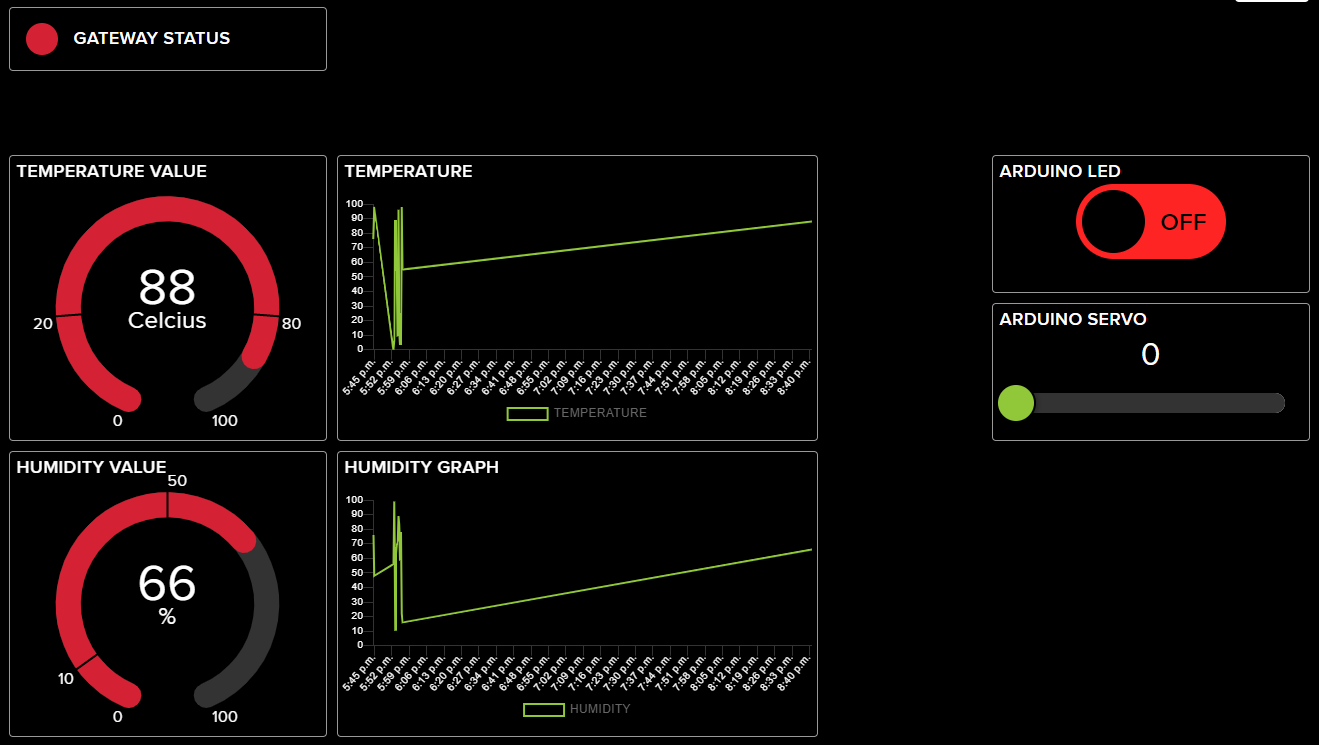
\includegraphics[scale=0.45]{screenshots/dashboard.png}
    \caption{Dashboard}
    \label{fig:dashboard}
\end{figure}

Figure \ref{fig:groups} captures the grouping feature of the Adafruit IO. Currently I have 2 groups, 1 is created default by the server, and 1 for this project. Grouping makes related topics more organized and eases the management of users. When a topic is assigned to a group other than the Default group, its proper name is prefix with its group name and a colon. 
\begin{figure}
    \centering
    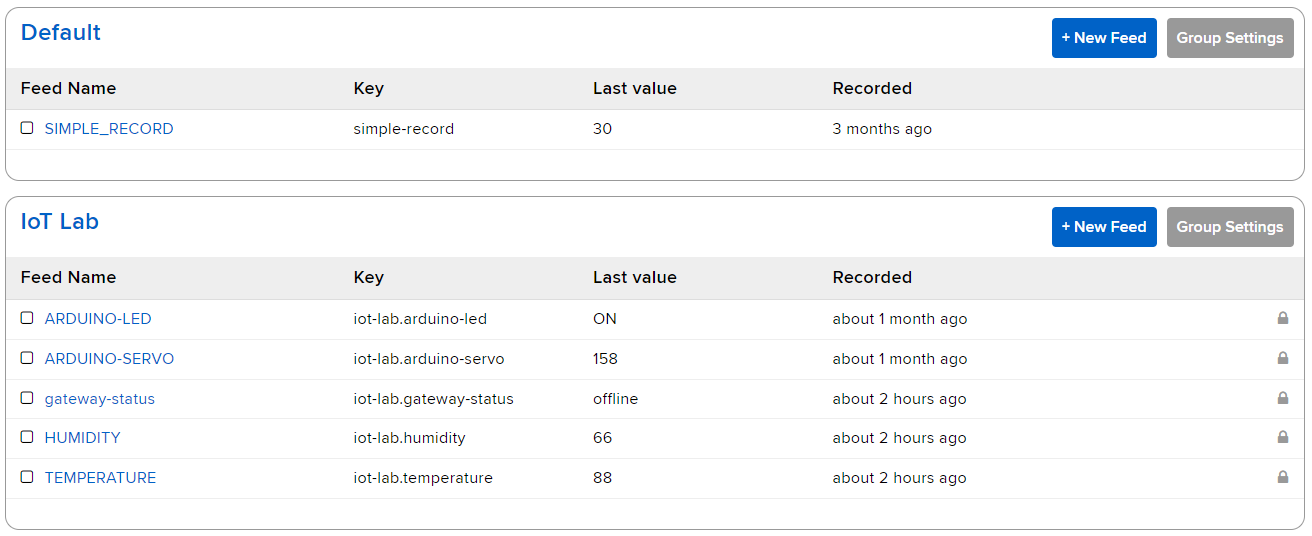
\includegraphics[scale=0.45]{screenshots/groups.png}
    \caption{Adafruit Grouping}
    \label{fig:groups}
\end{figure}
\clearpage
\section{Monitoring Application}
\label{mobile-application}
We hit another mother lode. This time we have to bring all the MQTT client implementation onto a mobile application. Most of the idea will be the same as what have been proposed for the gateway. I will spend more time discuss about modern mobile application development rather than digging into the MQTT. Let warm up with the Jetpack components.

\subsection{Jetpack Architecture}
Until recently, Google did not recommend a specific approach to building Android apps other than to provide tools and development kits while letting developers decide what worked best for a particular project or individual programming style. That changed in 2017 with the introduction of the Android Architecture Components which, in turn, became part of Android Jetpack when it was released in 2018. Android Jetpack consists of Android Studio, the Android Architecture Components and Android Support 
Library together with a set of guidelines that recommend how an Android App should be structured. The 
Android Architecture Components are designed to make it quicker and easier both to perform common tasks 
when developing Android apps while also conforming to the key principle of the architectural guidelines.

There are many components that makes up the Jetpack architecture, and our mobile application only use three: the \textit{ViewModel}, the \textit{Data Binding}, and the \textit{Navigation Graph}. They will be discussed shortly in upcoming sub-sections. Before moving on, it is important to understand the Jetpack approach to app development is not mandatory. While highlighting some of the shortcoming of other techniques that have gained popularity of the years, Google stopped short of completely condemning those approaches to app development. Google appears to be taking the position that while there is no right or wrong way to develop an app, there is a recommended way.

\subsubsection{Traditional Architecture}
An Android project typically consists of a single activity which contains all of the code for presenting and managing the user interface together with the back-end logic of the app. Up until the introduction of Jetpack, the most common architecture followed this paradigm with apps consisting of multiple activities (one for each screen within the app) with each activity class to some degree mixing user interface and back-end code.

This approach led to a range of problems related to the lifecycle of an app (for example an activity is destroyed and recreated each time the user rotates the device leading to the loss of any app data that had not been saved to some form of persistent storage) as well as issues such as inefficient navigation involving launching a new activity for each app screen accessed by the user.

At the most basic level, Google now advocates single activity apps where different screens are loaded as content within the same activity. Modern architecture guidelines also recommend separating different areas of responsibility within an app into entirely separate modules (a concept Google refers to as “separation of concerns”). One of the keys to this approach is the \textit{ViewModel} component.

\subsubsection{The ViewModel Component}
The purpose of ViewModel is to separate the user interface-related data model and logic of an app from the code responsible for actually displaying and managing the user interface and interacting with the operating system (Figure \ref{fig:viewmodel}). When designed in this way, an app will consist of one or more \textbf{UI Controllers}, such as an activity, together with ViewModel instances responsible for handling the data needed by those controllers.

In effect, the ViewModel only knows about the data model and corresponding logic. It knows nothing about the user interface and makes no attempt to directly access or respond to events relating to views within the user interface. When a UI controller needs data to display, it simply asks the ViewModel to provide it. Similarly, when the user enters data into a view within the user interface, the UI controller passes it to the ViewModel for handling.

This separation of responsibility addresses the issues relating to the lifecycle of UI controllers. Regardless of how many times a UI controller is recreated during the lifecycle of an app, the ViewModel instances remain in memory thereby maintaining data consistency. A ViewModel used by an activity, for example, will remain in memory until the activity completely finishes which, in the single activity app, is not until the app exits.

\begin{figure}
    \centering
    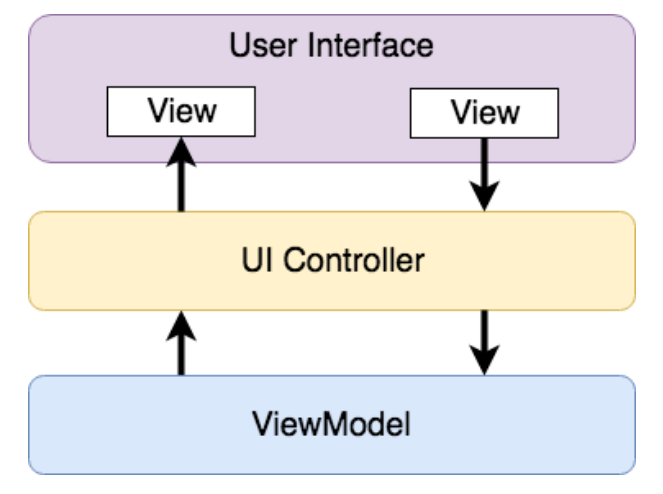
\includegraphics[scale=0.5]{screenshots/viewmodel.png}
    \caption{Jetpack Component - ViewModel}
    \label{fig:viewmodel}
\end{figure}

\subsubsection{LiveData and Data Binding}
Consider an app that displays realtime data such as the current price of a financial stock. There are only two ways that the UI controller can ensure that the latest data is displayed in the user interface. One option is for the controller to continuously check with the ViewModel to find out if the data has 
changed since it was last displayed. The problem with this approach, however, is that it is inefficient. To maintain the realtime nature of the data feed, the UI controller would have to run on a loop, continuously checking for the data to change.

A better solution would be for the UI controller to receive a notification when a specific data item within a ViewModel changes. This is made possible by using the \textit{LiveData} component. LiveData is a data holder that allows a value to become \textbf{observable} . In basic terms, an observable object has the ability to notify other objects when changes to its data occur thereby solving the problem of making sure that the user interface always matches the data within the ViewModel.

Another of the key advantages of using LiveData is that it is aware of the lifecycle state of its observers. If, for example, an activity contains a LiveData observer, the corresponding LiveData object will know when the activity’s lifecycle state changes and respond accordingly. If the activity is paused (perhaps the app is put into the background), the LiveData object will stop sending events to the observer. If the activity has just started or resumes after being paused, the LiveData object will send a LiveData event to the observer so that the activity has the most up to date value. Similarly, the LiveData instance will know when the activity is destroyed and remove the observer to free up resources.

Android Jetpack includes the Data Binding Library which allows data in a ViewModel to be mapped directly to specific views within the XML user interface layout file. Data binding allows the LiveData value stored in the ViewModel to be referenced directly within the XML layout file avoiding the need to write code to keep the layout views updated. Figure \ref{fig:data-binding} illustrates the idea.

\begin{figure}
    \centering
    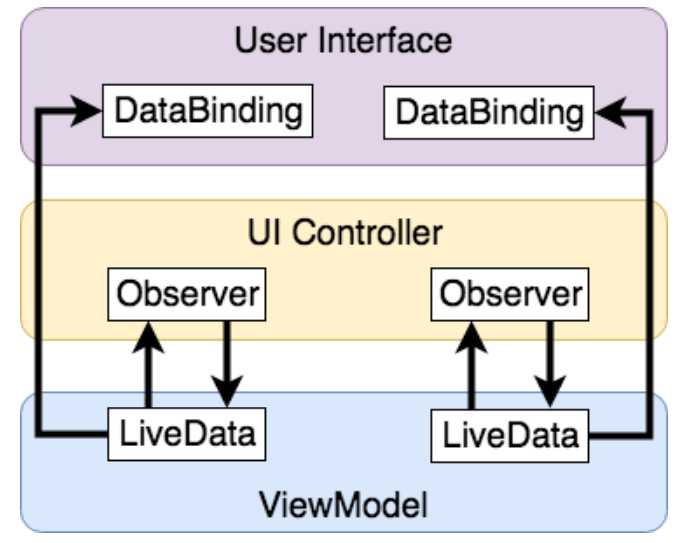
\includegraphics[scale=0.5]{screenshots/data binding.png}
    \caption{Jetpack Component - Data Binding}
    \label{fig:data-binding}
\end{figure}

\subsubsection{Navigation Graph}
Prior to the introduction of Android Jetpack, the implementation of navigation within an app was largely a manual coding process with no easy way to view and organize potentially complex navigation paths. This situation has improved considerably, however, with the introduction of the Android Navigation Architecture Component combined with support for navigation graphs in Android Studio.

A navigation graph is an XML file which contains the destinations that will be included in the app navigation. In addition to these destinations, the file also contains navigation actions that define navigation between destinations, and optional arguments for passing data from one destination to another. Android Studio includes a navigation graph editor that can be used to design graphs and implement actions either visually or by manually editing the XML. Figure \ref{fig:navigation-graph} shows the navigation graph of our mobile application.

\begin{figure}
    \centering
    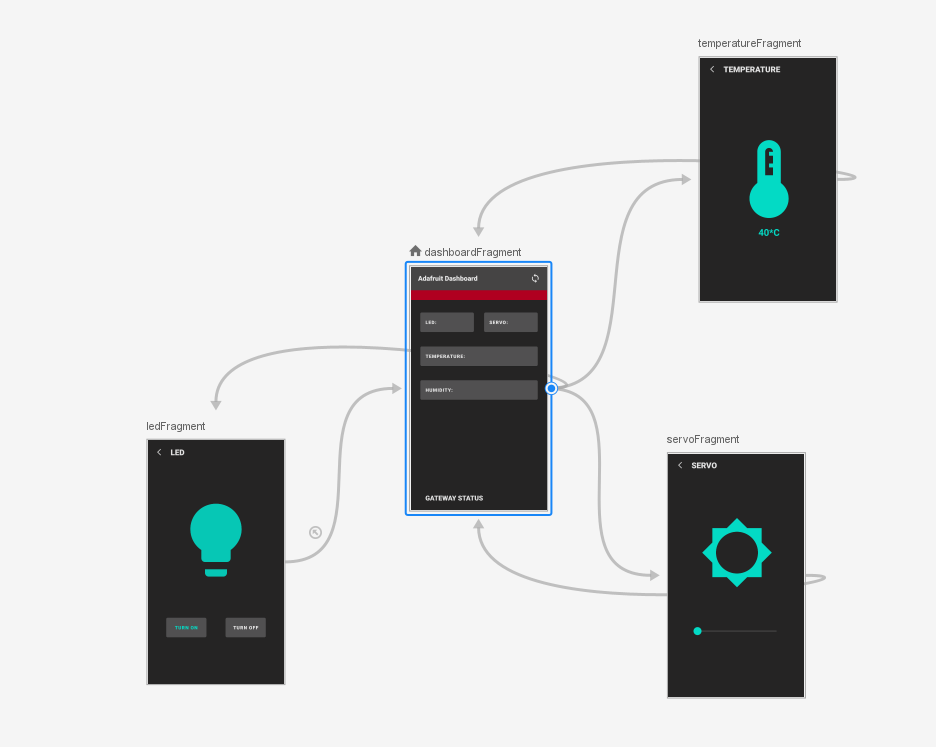
\includegraphics[scale=0.5]{screenshots/navigation_graph.png}
    \caption{Jetpack Component - Navigation Graph}
    \label{fig:navigation-graph}
\end{figure}

\subsection{MQTT in Mobile Application}
It would a pain if the implementation of our Android application is presented here. As I stated before, the project is hosted in this Github \href{https://github.com/hescul/adafruit-simple-iot}{\textcolor{blue}{repository}}, so it will be much more practical (and realistic) to pay it a visit. I will devote this section to explain how I achieve the MQTT protocol in an mobile app, together with modern components that we have come through. Listing \ref{code:mobile-main} shows the SIMPLIFIED version of the main activity class of our mobile app.
\begin{lstlisting}[language=Java, caption= Main Activity, escapeinside={(*}{*)}, label=code:mobile-main]
public class MainActivity extends AppCompatActivity
{
    // private fields
    // -----
    private MqttAndroidClient _client;
    private MqttConnectOptions _connectOptions;
    private DisconnectedBufferOptions _disconnectedBufferOptions;

    private DashboardViewModel _dashboardViewModel;


    // lifecycle methods
    // -----
    @Override
    protected void onCreate(@Nullable Bundle savedInstanceState) {
        super.onCreate(savedInstanceState);

        // inflate root view for this activity using view bing library
        setContentView(ActivityMainBinding.inflate(getLayoutInflater()).getRoot());

        // setup view model for fragments
        _dashboardViewModel = new ViewModelProvider(this).get(DashboardViewModel.class);

        // initialize and connect a client
        initClient();       (*\label{code:mobile-main:init}*)
        connectClient();    (*\label{code:mobile-main:connect}*)
    }

    @Override
    protected void onDestroy() {
        super.onDestroy();
        disconnectClient(); (*\label{code:mobile-main:disconnect}*)
    }

    // mqtt utilities
    // -----
    private void initClient() {
        final String serverURI = BrokerConfig.AUTH_CONTEXT + "://" + BrokerConfig.HOST_NAME + ':' + BrokerConfig.HOST_PORT;
        _client = new MqttAndroidClient(getApplicationContext(), serverURI, ClientConfig.CLIENT_ID);
        setupClient();
        setupCallback();
    }

    private void setupCallback() {
        _client.setCallback(new MqttCallbackExtended() {
            @Override
            public void connectComplete(boolean reconnect, String serverURI) {
                Timber.tag(logTag).d("Connected successfully: %s", serverURI);
            }

            @Override
            public void connectionLost(Throwable cause) {
                if (cause != null) {
                    Timber.tag(logTag).e("Lost connection to broker: %s", cause.getMessage());
                    _dashboardViewModel.setErrorMessage(cause.getMessage() + _dashboardViewModel.errorSuffix);
                    _dashboardViewModel.setConnected(false);
                }
            }

            @Override
            public void messageArrived(String topic, MqttMessage message) {
                Timber.tag(logTag).d("Received '%s' from %s", message, topic.substring(topic.indexOf('.') + 1));
                if (topic.contains(ClientConfig.SUBSCRIBE_TOPICS[ClientConfig.TOPICS.LED.ordinal()])) {             // led message
                    _dashboardViewModel.setLedStatus(message.toString());
                }
                else if (topic.contains(ClientConfig.SUBSCRIBE_TOPICS[ClientConfig.TOPICS.SERVO.ordinal()])) {      // servo message
                    _dashboardViewModel.setServoValue(message.toString());
                }
                else if (topic.contains(ClientConfig.SUBSCRIBE_TOPICS[ClientConfig.TOPICS.TEMPERATURE.ordinal()])) {// temperature message
                    _dashboardViewModel.setTemperatureValue(message.toString());
                }
                else if (topic.contains(ClientConfig.SUBSCRIBE_TOPICS[ClientConfig.TOPICS.HUMIDITY.ordinal()])) {   // humidity message
                    _dashboardViewModel.setHumidityValue(message.toString());
                }
                else if (topic.contains(ClientConfig.SUBSCRIBE_TOPICS[ClientConfig.TOPICS.STATUS.ordinal()])) {     // status message
                    _dashboardViewModel.setGtwStatus(message.toString());
                }
            }

            @Override
            public void deliveryComplete(IMqttDeliveryToken token) {
                try {
                    if (!token.getMessage().toString().isEmpty()) {
                        Timber.tag("mqtt").d("Delivered successfully (messageID = %d)", token.getMessageId());
                    }
                } catch (MqttException e) {
                    e.printStackTrace();
                }
            }
        });

    }

    private void setupClient() {
        // setup connection options
        _connectOptions = new MqttConnectOptions();
        _connectOptions.setUserName(BrokerConfig.USERNAME);
        _connectOptions.setPassword(BrokerConfig.PASSWORD.toCharArray());
        _connectOptions.setAutomaticReconnect(false);
        _connectOptions.setCleanSession(true);

        // setup disconnected buffer options
        _disconnectedBufferOptions = new DisconnectedBufferOptions();
        _disconnectedBufferOptions.setBufferEnabled(true);
        _disconnectedBufferOptions.setBufferSize(100);
        _disconnectedBufferOptions.setPersistBuffer(false);
        _disconnectedBufferOptions.setDeleteOldestMessages(false);
    }

    private void connectClient() {
        _dashboardViewModel.setConnecting(true);
        try {
            _client.connect(_connectOptions, null, new IMqttActionListener() {
                @Override
                (*\label{code:mobile-main:on-success}*)
                public void onSuccess(IMqttToken asyncActionToken) {
                    _client.setBufferOpts(_disconnectedBufferOptions);
                    subscribe();
                    fetchLatest();
                    _dashboardViewModel.setConnected(true);
                    _dashboardViewModel.setConnecting(false);
                }

                @Override
                public void onFailure(IMqttToken asyncActionToken, Throwable exception) {
                    Timber.tag(logTag).e("%s failed to reach %s: %s", ClientConfig.CLIENT_ID, BrokerConfig.HOST_NAME, exception.getMessage());
                    _dashboardViewModel.setErrorMessage(exception.getMessage() + _dashboardViewModel.errorSuffix);
                    _dashboardViewModel.setConnected(false);
                    _dashboardViewModel.setConnecting(false);
                }
            });
        } catch (MqttException e) {
            e.printStackTrace();
        }
    }

    private void disconnectClient() {
        if (_client.isConnected()) {
            try {
                IMqttToken token = _client.disconnect();
                token.setActionCallback(new IMqttActionListener() {
                    @Override
                    public void onSuccess(IMqttToken asyncActionToken) {
                        Timber.tag(logTag).d("%s disconnected successfully", ClientConfig.CLIENT_ID);
                    }

                    @Override
                    public void onFailure(IMqttToken asyncActionToken, Throwable exception) {
                        Timber.tag(logTag).e("%s failed to disconnect: %s", ClientConfig.CLIENT_ID, exception.getMessage());
                    }
                });

            } catch (MqttException e) {
                e.printStackTrace();
            }
        }
    }

    private void subscribe() {

        for (String topic : ClientConfig.SUBSCRIBE_TOPICS) {
            try {
                String realTopic = String.format("%s/feeds/%s.%s", BrokerConfig.USERNAME, ClientConfig.GROUP_KEY, topic);
                _client.subscribe(realTopic, 0, null, new IMqttActionListener() {
                    @Override
                    public void onSuccess(IMqttToken asyncActionToken) {

                    }

                    @Override
                    public void onFailure(IMqttToken asyncActionToken, Throwable exception) {
                        Timber.tag(logTag).e("Failed to subscribe to %s", topic);
                    }
                });
            } catch (MqttException e) {
                e.printStackTrace();
            }
        }
    }

    private void fetchLatest() {
        for (String topic : ClientConfig.SUBSCRIBE_TOPICS) {
            publish(String.format("%s/get", topic), "");
        }
    }
    private void fetchLatest(String topic) {
        publish(String.format("%s/get", topic), "");
    }

    private int publish(String topic, String msg) {
        String realTopic = String.format("%s/feeds/%s.%s", BrokerConfig.USERNAME, ClientConfig.GROUP_KEY, topic);
        int msgID = 0;
        try {
            IMqttToken token = _client.publish(realTopic, msg.getBytes(StandardCharsets.UTF_8), 0, false);
            token.setActionCallback(new IMqttActionListener() {
                @Override
                public void onSuccess(IMqttToken asyncActionToken) {

                }

                @Override
                public void onFailure(IMqttToken asyncActionToken, Throwable exception) {
                    Timber.tag("mqtt").e("Failed to publish %s to %s",msg ,topic);
                }
            });
            msgID = token.getMessageId();
        } catch (MqttException e) {
            e.printStackTrace();
        }
        return msgID;
    }
}
\end{lstlisting}
All the MQTT-things are gathered inside this class. The implementation may look different from that of in Python, but the overall idea is the same. When the host activity is created, we make the 2 calls to the \texttt{initClient()} and \texttt{connectClient()} function. They respectively construct an MQTT client instance and establish a connection for it to the broker (line \ref{code:mobile-main:init} and line \ref{code:mobile-main:connect}). When the activity get destroyed, we also disconnect the client from the server, as shown at line \ref{code:mobile-main:disconnect}. Another point that need pointed out is that we override the callback \texttt{onSuccess()} at line \ref{code:mobile-main:on-success} to have it subscribe to required topics and fetch latest data for us each time we successfully connect to the server.

And I think that's the main idea. Again, all the Android-related things can be found at this Github \href{https://github.com/hescul/adafruit-simple-iot}{\textcolor{blue}{repository}}. Overall it's kinda fun to work with mobile, it really shapes up the organization mindset for the developers.
\clearpage
\section{Conclusion}
It's time to wrap things up. I must say this seemingly small-scaled project gave me much more of what I expected. It may hard to catch up at first but when the pace is maintained, one could push it far beyond expectation. After all, I would like to give my professor, Mr. Nhan, a big thankful appreciation, for his wonderful dedication to the teaching of this course. 
\clearpage

%%%%%%%%%%%%%%%%%%%%%%%%%%%%%%%%%
\addcontentsline{toc}{section}{Reference}
\begin{thebibliography}{99999}

\bibitem[Web]{1}{Arduino,} {\url{https://www.arduino.cc/}}

\bibitem[Web]{2}{MQTT Retained Message,} {\url{http://bitly.ws/mvqS}}

\bibitem[Web]{3}{MQTT QoS,} {\url{http://bitly.ws/mvr4}}

\bibitem[Book]{4}{Neil Symth,} {Android Studio 4.2 Development Essentials - Java Edition}

\end{thebibliography}
\end{document}
